\part{复分析学}
\chapter{复分析}
\section{考试内容}
\subsection{正规族}
\begin{defi}[正规族]\label{def: normal family}
    设 $\mathscr{F}=\{f_\alpha \colon D\to \mathbb{C}\mid \alpha \in A\}$是区域 $D$上的一个解析函数族. 我们称 $\mathscr{F}$是一个正规族 (normal family),\textbf{如果 $\mathscr{F}$中的任意序列都包含一个子序列,该子序列在 $D$ 内局部一致收敛.}
\end{defi}
\begin{thm}[Montel 定理]\label{thm: Montel thm}
    设 $\mathscr{F}=\{f_\alpha \colon D\to \mathbb
    {C} ,\alpha\in A\}$ 是区域 $D$ 上的一个解析函数族. 若对于 $D$ 中的任意一个紧子集 $E\subset D$ , $f_\alpha$ 在 $E$ 上是一致有界的, 则 $\mathscr{F}$在 $D$ 上是正规族.
\end{thm}
\begin{proof}
    对于任意给定的紧子集 $E$, 我们取 $\delta_0>0$ 充分小,使集合
$$
E_0=\left\{z \in \mathbb{C}: d(z, E) \leqslant 2 \delta_0\right\} \subset D,
$$
其中 $d(z, E)$ 是 $z$ 到 $E$ 的距离. 根据定理的假定, 对于紧子集 $E_0$ 存 在一数 $M$,使得
$$
\left|f_\alpha(z)\right| \leqslant M, \quad \forall z \in E_0, \alpha \in A .
$$
由 Cauchy 不等式有
$$
\left|f_a^{\prime}(z)\right| \leqslant \frac{M}{\delta_0}, \quad \forall z \in E, \alpha \in A .
$$
这意味着
$$
\left|f_\alpha\left(z_1\right)-f_\alpha\left(z_2\right)\right| \leqslant \frac{M}{\delta_0}\left|z_1-z_2\right|, \quad \alpha \in A,
$$
只要 $z_1, z_2 \in E$ 且 $\left|z_1-z_2\right|<\delta_0$. 这样, $f_a$ 在 $E$ 上等度连续. 由 Arzela 定理就推出本定理. 
\end{proof}
\begin{thm}[Riemann 映射定理]\label{thm: Riemann map theorem}
    设 $D\subset \mathbb
    {C}$ 是一个单连通区域,且其边界点多于一点.又设 $z_0\in D$ 是任意给定的一点,则存在一个共形映射 $\varphi : D\to \Delta$ ,将 $D$映为单位圆周 $\Delta$, $\varphi(z_0)=0$,
    且 $\varphi^\prime (z_0)>0$,这样的映射 $\varphi$ 是唯一的.
\end{thm}
\begin{proof}
    设 $\mathscr{F}=\{f\colon D\to \Delta\}$ 是全体在 $D$ 上单叶且将 $D$ 映入 $\Delta$ 内的解析函数族.

    首先, 我们证明 $\mathscr{F}\neq \emptyset$. 设 $a,b\in \partial D$, 且 $a\neq b$. 令
    $$
g(z)=\frac{z-a}{z-b},
$$
那么,区域 $D^{\prime}=g(D)$ 是一个不包含 0 与 $\infty$ 的单连通域, 且其边界 $\partial D^{\prime}$ 包含 0 及 $\infty$. 于是, 函数 $w=\sqrt{g}$ 在 $D$ 中有两个单值解析分支, 分别记为 $h_{+}(z)$ 及 $h_{-}(z)$, 且满足
$$
h_{+}(z)=-h_{-}(z), \quad \forall z \in D .
$$
这样 $h_{+}(D)$ 与 $h_{-}(D)$ 是关于原点对称的两个区域 (见\textbf{图~\ref{fig:riemann mappings}}).
\begin{figure}[ht]
    \centering
    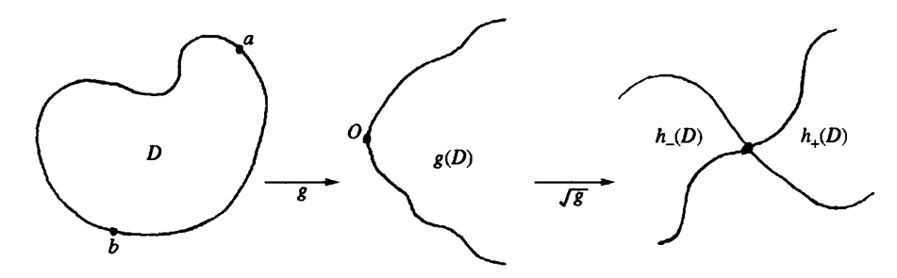
\includegraphics{figures/riemann mapping thm.png}
    \caption{\textbf{Riemann映射定理}}
    \label{fig:riemann mappings}
\end{figure}
在 $h_{-}(D)$ 中取一点 $w_0$, 并假定以 $w_0$ 为圆心、以 $\delta>0$ 为半径的 圆完全包含于 $h_{-}(D)$ 之中. 这时函数
$$
f_*(z)=\frac{\delta}{h_{+}(z)-w_0}
$$
则在 $\mathscr{F}$ 之中.
现在, 我们考虑这样的极值问题: 在 $\mathscr{F}$ 中求一函数使其在 $z_0$ 点的导数的模最大.
设 $r>0$ 使得 $\Delta_r\left(z_0\right) \subset D$. 这时根据 Cauchy 不等式及单叶性,
$$
0<\left|f^{\prime}\left(z_0\right)\right| \leqslant \frac{1}{r}, \quad \forall f \in \mathscr{F} .
$$
令
$$
\alpha=\sup \left\{\left|f^{\prime}\left(z_0\right)\right|: f \in \mathscr{F}\right\} .
$$
由 $\left|f_*^{\prime}\left(z_0\right)\right|>0$ 可知 $\alpha>0$. 显然, 存在 $f_n \in \mathscr{F}(n=1,2, \cdots)$, 使得
$$
\left|f_n^{\prime}\left(z_0\right)\right| \geqslant \alpha-\frac{1}{n} \text {. }
$$
由 Montel 定理, $\mathscr{F}$ 是一个正规族. 这样, 在序列 $\left\{f_n\right\}$ 中存在一 个子序列 $\left\{f_{n_k}\right\}$ 在 $D$ 内局部一致收敛. 设其极限为 $f_0$, 那么, 根据
Weierstrass 定理, $f_0$ 是 $D$ 上的解析函数, 且 $\left|f_0^{\prime}\left(z_0\right)\right|=\alpha$.

又因为 $f_n$ 是单叶的, 根据 $\S 2$ 中的定理 $2, f_0$ 要么是单叶的, 要 么是常数. 注意到 $\alpha>0$, 可知后一种情况不可能. 故 $f_0$ 是单叶函数, 且 $\left|f_0\right|<1$.

这样, 我们证明了在 $\mathscr{F}$ 中存在一个 $f_0$, 使其在 $z_0$ 点的导数的模 达到最大.

现在, 我们要进一步证明 $f_0\left(z_0\right)=0$ 且 $f_0$ 将 $D$ 变为 $\Delta$. 

假定 $f_0\left(z_0\right)=\beta \neq 0$. 令
$$
f_1(z)=\frac{f_0(z)-\beta}{1-\bar{\beta} f_0(z)},
$$
则显然 $f_1 \in \mathscr{F}$. 简单计算表明
$$
f_1^{\prime}\left(z_0\right)=\frac{f_0^{\prime}\left(z_0\right)}{1-\bar{\beta} \beta} .
$$
于是, $\left|f_1^{\prime}\left(z_0\right)\right|>\left|f_0^{\prime}\left(z_0\right)\right|$, 与 $\left|f_0^{\prime}\left(z_0\right)\right|$ 的最大性矛盾. 由此推出
$$
f_0\left(z_0\right)=0 .
$$
假定 $f_0(D)$ 不是 $\Delta$, 即存在一点 $w_1 \in \Delta \backslash f_0(D)$. 这时, 函数
$$
\psi(z)=\frac{f_0(z)-w_1}{1-\bar{w}_1 f_0(z)} \quad(z \in D)
$$
不取 0 及 $\infty$. 因此, $\sqrt{\psi}$ 在 $D$ 内有单值解析分支, 设其为 $h$. 则 $h \in\mathscr{F}$.
又令
$$
f_2(z)=\frac{h(z)-h\left(z_0\right)}{1-\overline{h\left(z_0\right)} h(z)},
$$
则 $f_2 \in \mathscr{F}$. 经过计算, 我们有
$$
f_2^{\prime}\left(z_0\right)=\frac{-\left(1+\left|w_1\right|\right)}{2 \sqrt{w_1}} f_0^{\prime}\left(z_0\right) .
$$
再次导致 $\left|f_0^{\prime}\left(z_0\right)\right|$ 不是最大的, 产生矛盾. 由此推出: $f_0(D)=\Delta$.

总之, 我们证明了 $f_0: D \rightarrow \Delta$ 是 $D$ 到 $\Delta$ 的共形映射, 且 $f_0\left(z_0\right)=0$. 显然, 取适当的 $\theta \in \mathbb{R}$ 可使 $\varphi=\mathrm{e}^{\mathrm{i} \theta} f_0$ 满足定理要求: $\varphi^{\prime}\left(z_0\right)>0$. 

下面证明映射的惟一性. 假如另有一个 $D$ 到 $\Delta$ 的共形映射 $\tilde{\varphi}: D \rightarrow \Delta, \tilde{\varphi}\left(z_0\right)=0$ 且 $\tilde{\varphi}^{\prime}\left(z_0\right)>0$. 那么 $\varphi^{\circ} \circ \varphi^{-1}$ 是 $\Delta$ 的解析自同构映
射, 且将 $0$ 变为 $0$ . 因此, $\tilde{\varphi} \circ \varphi^{-1}=\mathrm{e}^{\mathrm{i} \theta} z, \theta \in \mathbb{R}$. 由条件 $\varphi^{\prime}\left(z_0\right)>0$ 及 $\tilde{\varphi}\left(z_0\right)>0$, 立即推出 $\mathrm{e}^{\mathrm{i} \theta}=1$, 也即 $\tilde{\varphi}=\varphi$. 这样, 我们完成了定理中的 唯一性部分的证明.
\end{proof}
Riemann 映射定理使我们得以对 $\overline{\mathbb{C}}$ 上的单连通域, 进行解析同 构分类:
\begin{thm}
    设 $D$ 为 $\overline{\mathbb{C}}$ 上的单连通区域, 则 $D$ 解析同构于下列三种区域之一 : $,\overline{\mathbb{C}}, \mathbb{C}$, 或 $\Delta$. 上述三种区域之间两两互不解析同构.
\end{thm}
\begin{proof}
    证明是容易的. 事实上, 若区域 $D$ 不是 $\overline{\mathbb{C}}$ 且仅有一个边界点, 那 么可以通过一个分式线性变换将该边界点变为 $\infty$, 而这时 $D$ 则变为 $\mathbb{C}$. 若区域 $D$ 的边界点多于一点, 则通过一个分式线性变换使 $D$ 的 像成为 $\mathbb{C}$ 中的单连通域, 且其边界点多于一点; 从而可应用 Riemann 映射定理.
这里我们要进一步指出, $\overline{\mathbb{C}}, \mathbb{C}$ 与 $\Delta$ 中两两互不解析同构.
事实上, $\mathbb{\mathbb { C }}$ 是紧的, 而 $\mathbb{C}$ 与 $\Delta$ 是非紧的. 故 $\mathbb{\mathbb { C }}$ 与 $\mathbb{C}$ 或 $\Delta$ 不拓扑 等价, 因而不可能解析同构. 另外, 由 Liouville 定理可知, 任意一个 解析函数 $f: \mathbb{C} \rightarrow \Delta$ 只能是常数, 这表明 $\mathbb{C}$ 与 $\Delta$ 不可能解析同构.
\end{proof}
现在, 我们利用模函数及单值性定理来证明 Picard 小定理.
\begin{thm}[Picard 定理]\label{thm: Picard thm}
设 $f(z)$ 是一个整函数, 即在 $\mathbb{C}$ 上解析的 函数. 若存在两点 $a$ 与 $b, a \neq b$, 使得
$$
f(z) \neq a \text { 和 } b, \quad \forall z \in \mathbb{C},
$$
则 $f$ 是常数.
这就是说, 非常数的整函数至多有一个例外值取不到. 有一个例 外值的非常数的整函数是存在的, 例如 $w=\mathrm{e}^z$.
\end{thm}
\begin{proof}
不失一般性, 可设 $a=0, b=1$.
设 $\lambda$ 是模函数 $\mu$ 的反函数. 它是一个多值解析函数, 但在任意一 点附近可以取到单值解析分支. 设 $w_0 \in f(\mathbb{C})$, 则 $w_0 \neq 0,1$. 那么, 可 以在 $w_0$ 的一个邻域内取到 $\lambda$ 的一个单值分支, 仍记为 $\lambda$.

我们考虑复合函数 $\lambda \circ f$. 它在点 $z_0$ 的附近是一个单值解析函 数, 其中 $f\left(z_0\right)=w_0$. 设 $P_0$ 是 $\lambda \circ f$ 在 $z_0$ 处的幂级数展开式. 那么, $P_0$ 在 $\mathbb{C}$ 上沿任意一条路径均可延拓. 要说明这一点只要注意到 $\mu$ 是 一覆盖映射即可, 请读者自行验证.

复平面 $\mathbb{C}$ 是单连通域. 由单值性定理, 即推出 $P_0$ 延拓的结果在 $\mathbb{C}$ 上定义了一个单值解析函数, 记为 $F$. 那么, $|F(z)|<1, \forall z \in \mathbb{C}$. 由 Liouville 定理, $F$ 是常数, 从而 $f$ 是常数. 
\end{proof}

\begin{thm}[Bieberbach 定理]\label{thm: Bieberbach}
    设
    \begin{eq*}
        f(z)=z+a_2 z^2+\cdots,
    \end{eq*}
    是 $S$ 类中的函数,则 $|a_2|\leqslant 2$.
\end{thm}
\begin{thm}[Kobe  $\frac 14$ 定理]\label{thm : Kobe theorem}
    设 $f$ 是单位圆 $\Delta$ 内的单叶函数, 且 $f(0) =0,f^\prime (0)=1 $, 则 $f(\Delta)$包含圆
    \[\left\{w\colon |w|<\frac{1}{4} \right\}.\]
\end{thm}
\begin{proof}
    设 $c$ 不在 $f(\Delta)$ 之内, 则 $c \neq 0$ 且函数
$$
f_1(z)=\frac{c f(z)}{c-f(z)}=z+\left(a_2+\frac{1}{c}\right) z^2+\cdots,
$$
其中 $a_2$ 为 $f$ 的展开式中的系数. 显然, $f_1$ 是 $S$ 类函数. 于是由 Bieberbach 定理有
$$
\left|a_2+\frac{1}{c}\right| \leqslant 2,
$$
也即
$$
\frac{1}{|c|} \leqslant 2+\left|a_2\right| \leqslant 4 \text {. }
$$
\end{proof}

\begin{thm}[偏差定理] \label{thm: piancha theorem}
    设 $f\in S$, 则有估计式
    \[\frac{|z|}{(1+|z|)^2}\leqslant |f(x)|\leqslant \frac{|z|}{(1-|z|)^2}, \quad\forall z\in \Delta .\]
\end{thm}
\begin{proof}
    证明有一定的技巧性. 令 $z$ 为 $\Delta$ 内一固定点, 并考虑函数
$$
f_1(\zeta)=\frac{f\left(\frac{\zeta+z}{1+\bar{z} \zeta}\right)-f(z)}{\left(1-|z|^2\right) f^{\prime}(z)} .
$$
显然, $f_1$ 是 $\zeta \in \Delta$ 的单叶函数, 且 $f_1(0)=0, f_1^{\prime}(0)=1$, 故 $f_1 \in S$. 由 计算得
$$
f_1^{\prime \prime}(0)=\left(1-|z|^2\right) \frac{f^{\prime \prime}(z)}{f^{\prime}(z)}-2 \bar{z} .
$$
由 Bieberbach 定理有 $\left|f_1^{\prime \prime}(0) / 2\right| \leqslant 2$, 也即
$$
\left|\frac{z f^{\prime \prime}(z)}{f^{\prime}(z)}-\frac{2 r^2}{1-r^2}\right| \leqslant \frac{4 r}{1-r^2}, \quad|z|=r .
$$
注意到
$$
\operatorname{Re} \frac{z f^{\prime \prime}(z)}{f^{\prime}(z)}=r \frac{\partial}{\partial r} \ln \left|f^{\prime}(z)\right|,
$$
我们有
$$
\frac{-4+2 r}{1-r^2} \leqslant \frac{\partial}{\partial r} \ln \left|f^{\prime}(z)\right| \leqslant \frac{4+2 r}{1-r^2} .
$$
对 $r$ 积分即得
$$
\frac{1-r}{(1+r)^3} \leqslant\left|f^{\prime}(z)\right| \leqslant \frac{1+r}{(1-r)^3} .
$$
再对 $r$ 积分即得我们所要的关于 $|f(z)|$ 的上界估计式.
为了得到 $|f(z)|$ 的下界估计式, 我们考虑以 0 为圆心过 $z$ 点所 作的圆周 $\Gamma$. 设 $z_1 \in \Gamma$ 使 $\{|f(z)|: z \in \Gamma\}$ 达到最小, 并用直线段 $\beta$ 连 结 $f\left(z_1\right)$ 与 $f(0)=0$. 记 $f^{-1}(\beta)$ 为 $\alpha$, 则有
$$
\begin{aligned}
|f(z)| & \geqslant\left|f\left(z_1\right)\right|=\int_\alpha\left|f^{\prime}(t)\right||\mathrm{d} t| \\
& \geqslant \int_\alpha \frac{1-|t|}{(1+|t|)^3}|\mathrm{~d} t| \geqslant \int_0^r \frac{1-\eta}{(1+\eta)^3} \mathrm{~d} \eta \\
& =\frac{r}{(1+r)^2} \quad(r=|z|) .
\end{aligned}
$$
\end{proof}
\begin{prop}
    在单位圆解析自同构映射下, Poincar\'{e} 距离不变.
\end{prop}
\begin{proof}
    事实上只要证明 Poincaré 度量在 $\Delta$ 的自同构映射下不变 即可.
设 $f \in \operatorname{Aut}(\Delta)$, 也即 $f$ 是保持单位圆 $\Delta$ 不变的分式线性变换:
$$
f(z)=\mathrm{e}^{\mathrm{i} \alpha} \frac{z-a}{1-\bar{a} z}, \quad a \in \Delta, \alpha \in \mathbb{R} .
$$
那么, 我们有
$$
f^{\prime}(z)=\mathrm{e}^{\mathrm{i} \alpha} \frac{1-|a|^2}{(1-\bar{a} z)^2} .
$$
简单计算表明
$$
\frac{\left|f^{\prime}(z)\right|}{1-|f(z)|^2}=\frac{1}{1-|z|^2},
$$
于是我们得到
$$
\frac{2|\mathrm{~d} w|}{1-|w|^2}=\frac{2|\mathrm{~d} z|}{1-|z|^2}, \quad w=f(z) .
$$
由此推出, 任意一条可求长曲线 $\gamma$ 与它的像 $f(\gamma)$ 有相同的 Poincaré 长度, 从而 $f$ 保持 $\Delta$ 中 Poincaré 距离不变.
\end{proof}
\begin{thm}[Schwarz 引理] \label{thm: Schwarz lem}
    设 $f$ 是单位圆 $\Delta$ 内的解析函数, 且 $f(\Delta)\subset \Delta, f(0)=0$, 则 $|f^\prime (0)|\leqslant 1$, 且 $|f(z)|\leqslant |z|,\forall z\in \Delta$. 若 $|f^\prime (0)|=1$或 对一点 $z_0\in \Delta\backslash \{0\}$ 有 $|f(z_0)|=|z_0|$, 则 $f(z)\equiv e^{i\theta}z$,其中 $\theta\in \mathbb{R}$是常数.
\end{thm}
\begin{thm}[Schwarz--Pick 定理]\label{thm: Schwarz - pick thm}
    设 $f$ 是单位圆 $\Delta$ 内的解析函数, 且 $f(\Delta)\subset \Delta$. 又设 $d(\bullet,\bullet)$ 表示 $\Delta$ 内两点间的Poincar\'{e}距离, 则有
    \[d(f(z_1),f(z_2))\leqslant d(z_1,z_2),\quad\forall z_1,z_2\in \Delta,\]
    这里等号对任意两个不同点 $z_1$ 与 $z_2$ 成立的充要条件是
    \[f\in \operatorname{Aut} (\Delta).\]
\end{thm}
\begin{proof}
    令 $g$ 是将 $z_1$ 变为 0 且保持 $\Delta$ 不变的分式线性变换, $h$ 是将 $f\left(z_1\right)$ 变为 0 且保持 $\Delta$ 不变的分式线性变换. 我们考虑函数 $F=h \circ f \circ g^{-1}$, 则 $F$ 是 $\Delta$ 内的解析函数, $F(0)=0$, 且 $F(\Delta) \subset \Delta$. 应用 Schwarz 引理, 我们有
$$
\left|F\left(\zeta_2\right)\right| \leqslant\left|\zeta_2\right|, \quad \zeta_2=g\left(z_2\right) .
$$
Pick 将此式解释为
$$
d\left(0, F\left(\zeta_2\right)\right) \leqslant d\left(0, \zeta_2\right),
$$
也即
$$
d\left(h \circ f\left(z_1\right), h \circ f\left(z_2\right)\right) \leqslant d\left(g\left(z_1\right), g\left(z_2\right)\right) .
$$
由 $\S 1$ 中的命题 1 立即推出:
$$
d\left(f\left(z_1\right), f\left(z_2\right)\right) \leqslant d\left(z_1, z_2\right) .
$$
关于等号成立的条件可由 Schwarz 引理中相应部分推得.
\end{proof}
\begin{defi}[Poincar\'{e}度量]
    \textbf{\color{magenta} 单位圆 $\Delta$ }的Ponicar\'{e}度量可写成 $\dd s=\rho_\Delta (z) |\dd z|$, 其中
    \[\rho_\Delta (z)=\frac{2}{1-|z|^2}\]
    称为Poncar\'{e}度量的\textbf{密度}. 上述定理可写成\textbf{微分形式}:
    \[\rho_\Delta (f(z))|f^\prime (z)|\leqslant \rho_\Delta (z),\quad\forall z\in \Delta.\]

    $\color{purple}{\overline{\mathbb{C}}\backslash \{0,1,\infty\}}$的Poincar\'{e}度量的局部表示式为
    \[\dd s=\frac{2|\lambda^\prime(z)|}{1-|\lambda(z)|^2}|\dd z|
    \]
    其中$\lambda$为 $\mu$的反函数的一个单值分支.
\end{defi}
\begin{thm}[广义Schwarz引理]\label{thm: extension of Schwarz lem}
    设区域 $D$ 与 $G$ 均具有单位圆 $\Delta$ 到它们的全纯覆盖映射, 其Poincar\'{e}度量分别为
    \begin{align*}
        \dd s_1 &=\sigma_1 (z) |\dd z|,z\in D;\\ 
        \dd s_2 &=\sigma_2 (w) |\dd w|,w\in G.
    \end{align*}
    又设 $f\colon D\to G$是全纯映射,则
    \[\sigma_2 (f(z))|f^\prime (z)|\leqslant \sigma_1 (z),z\in D,\]
    其中等号在一点成立的充要条件是 $f$是 $D$ 到 $G$ 的覆盖映射.
\end{thm}
\begin{proof}
    设 $h_1: \Delta \rightarrow D$ 与 $h_2: \Delta \rightarrow G$ 是全纯覆盖映射. 对于任意一点 $z_0 \in D$ 及 $w_0=f\left(z_0\right) \in G$, 我们分别取它们的小邻域 $U$ 及 $V$, 使得 $h_1^{-1}$ 及 $h_2^{-1}$ 分别在 $U$ 及 $V$ 上有单值分支. 我们将它们记为 $\varphi: U \rightarrow U_1$ 及 $\psi: V \rightarrow V_1$, 并考虑函数
    \begin{eq*}
        F=\psi\circ f\circ \varphi^{-1}.
    \end{eq*}
只要 $U$ 取得充分小使得 $f(U) \subset V$, 则上述 $F$ 是有意义的.
$F$ 是定义在 $U_1$ 上一个解析函数. 它显然可以沿 $\Delta$ 内的任意一 条路径进行解析延拓, 所得的结果是一个单值解析函数, 仍记为 $F$. 设 $\zeta_0 \in U_1$ 使得 $h_1\left(\zeta_0\right)=z_0$. 又记 $\eta_0=F\left(\zeta_0\right)$. 对 $F: \Delta \rightarrow \Delta$ 使用 Schwarz-Pick 定理(微分形式), 则有
$$
\rho_{\Delta}\left(F\left(\zeta_0\right)\right)\left|F^{\prime}\left(\zeta_0\right)\right| \leqslant \rho_{\Delta}\left(\zeta_0\right),
$$
也即 $\rho_{\Delta}\left(\eta_0\right)\left|\psi^{\prime}\left(w_0\right)\right| \cdot\left|f^{\prime}\left(z_0\right)\right|\left|h_1^{\prime}\left(\zeta_0\right)\right| \leqslant \rho_{\Delta}\left(\zeta_0\right)$. 此式可以改写成
$$
\rho_{\Delta}\left(\eta_0\right)\left|\psi^{\prime}\left(w_0\right)\right| \cdot\left|f^{\prime}\left(z_0\right)\right| \leqslant \rho_{\Delta}\left(\zeta_0\right)\left|\varphi^{\prime}\left(z_0\right)\right| .
$$
根据 Poincaré 度量的定义, 我们有
$$
\sigma_2\left(f\left(z_0\right)\right)\left|f^{\prime}\left(z_0\right)\right| \leqslant \sigma_1\left(z_0\right) .
$$
当等号成立时, $F \in \operatorname{Aut}(\Delta)$. 这时, 由 $h_2 \circ F=f \circ h_1$ 得
$$
h_2=f \circ h_1 \circ F^{-1} \text {. }
$$
由此又可推出 $f$ 是局部单叶的满射, 并满足覆盖映射的条件.
\end{proof}

\begin{proof}{(用广义Schwarz引理证明Picard小定理)}

    设 $f\colon \mathbb{C}\to \mathbb{C}\backslash \{0,1\} $是一个解析函数.用 $\rho_{0,1}(z)|\dd z|$表示 $\mathbb{C}\backslash \{0,1\}$的Poincar\'{e}度量.另外很容易算出 $\Delta_r (0)=\{z\colon |z|<r\}$的Poincar\'{e}度量是
    \[\dd s=\frac{2r|\dd z|}{r^2-|z|^2}.\]
    将 $f$视为 $\Delta_r (0)\to \mathbb{C}\backslash\{0,1\}$的解析函数,并应用广义Schwarz引理即得
    \[\rho_{0,1}(f(z))|f^\prime (z)|\leqslant \frac{2r}{r^2-|z|^2},\quad\forall z\in \Delta_r (0).\]
    令 $r\to\infty$即可推出 $f^\prime (z)=0$,从而 $f$ 是常数.
\end{proof}
\begin{thm}\label{thm:thm1}
    设 $\dd s=\rho |\dd z|$是单位圆 $\Delta$ 上的Poincar\'{e}度量,而 $\dd s=\sigma|\dd z|$是 $\Delta$上的一个度量, $\sigma>0,\sigma\in C^2$,且 $K(\sigma)\leqslant -1$, 则有
    \[\rho(z)\geqslant \sigma(z),\quad\forall z\in \Delta.\]
\end{thm}
\begin{proof}
    首先假定 $\sigma$ 在 $\bar{\Delta}$ 上连续, 且在单位圆周上严格大于 0 . 我们 考虑函数
$$
F=\ln \rho-\ln \sigma .
$$
显然, 当 $|z| \rightarrow 1$ 时 $F(z) \rightarrow+\infty$. 因此, $F$ 在 $\Delta$ 内达到最小值. 设在 $z_0$ 点达到 $F$ 的最小值. 假若其最小值 $F\left(z_0\right)<0$, 则
$$
\begin{aligned}
\left.\Delta F\right|_{z_0} & =\left.\Delta(\ln \rho-\ln \sigma)\right|_{z_0} \\
& \leqslant\left.\left(\rho^2-\sigma^2\right)\right|_{z_0}<0,
\end{aligned}
$$
这与 $z_0$ 是极小值稳定点矛盾. 因此, 最小值 $F\left(z_0\right) \geqslant 0$, 也即 $\rho(z) \geqslant$ $\sigma(z), \forall z \in \Delta$.
现在, 我们去掉 $\sigma$ 在 $\bar{\Delta}$ 上连续的限制. 令 $\sigma_r=r \sigma(r z), 0<r<1$. 这时对 $\sigma_r$ 应用上述结论即有 $\rho(z) \geqslant r \sigma(r z)$. 令 $r \rightarrow 1$ 即完成定理之 证明.
\end{proof}
\begin{thm}
    设 $D$ 是一个区域, $\dd s=\sigma_j |\dd z|$为 $D$内的度量, $\sigma_j>0,\sigma_j\in C^2,j=1,2$, 并且满足
    \[K(\sigma_1)=-1,K(\sigma_2)\leqslant -1,\]
    且对任意边界点 $\zeta$ 都有
    \[\lim_{z\to\zeta}\inf \frac{\sigma_1 (z)}{\sigma_2 (z)}\geqslant 1,\]
    则有
    \[\sigma_1 (z)\geqslant \sigma_2 (z),\quad\forall z\in D.\]
\end{thm}
\begin{proof}
    证明与\textbf{定理~\ref{thm:thm1}} 一致.
\end{proof}
\begin{thm}[比较定理]\label{thm: compare thm}
    设 $\Gamma_1$与 $\Gamma_2$为两个局部可求长曲线族. 若 $\Gamma_1$中的每条曲线 $\gamma_1$都包含 $\Gamma_2$中的一条曲线 $\gamma_2$,则 $\lambda (\Gamma_1)\geqslant \lambda (\Gamma_2)$.
\end{thm}

\begin{thm}[合成原理]
    设 $\Gamma,\Gamma_1$和 $\Gamma_2$是三个局部可求长曲线族, 且 $\Gamma_1$与 $\Gamma_2$中的曲线分别包含于区域 $D_1$与 $D_2$中, $D_1 \bigcap D_2=\emptyset$.则有
    \begin{enumerate}[label=(\roman*),font=\upshape]
        \item 若 $\Gamma_1$中的每一条曲线 $\gamma_1$与 $\Gamma_2$中的每一条曲线 $\gamma_2$都包含 $\Gamma$中的某条曲线 $\gamma$, 那么
        \[\frac{1}{\lambda (\Gamma)}\geqslant \frac{1}{\lambda (\Gamma_1)}+\frac{1}{\lambda (\Gamma_2)};\]
    \item 若 $\Gamma$中的每条曲线 $\gamma$都包含 $\Gamma_1$中的某条曲线 $\gamma_1$与 $\Gamma_2$中的某条曲线 $\gamma_2$,那么
    \[\lambda (\Gamma)\geqslant\lambda (\Gamma_1)+\lambda (\Gamma_2).\]
    \end{enumerate}
\end{thm}

\begin{thm}
    设 $Q(z_1,z_2,z_3,z_4)$ 是一拓扑四边形. 又设 $\Gamma$是 $Q$中第一组对边之间的所有局部可求长连线所组成的曲线族,则有
    \[\operatorname{Mod} (Q(z_1,z_2,z_3,z_4))=\frac{1}{\lambda(\Gamma)}.\]
\end{thm}
\begin{proof}
    因为共形模与极值长度都是共形不变量,所以不失一般性可设 $Q$ 是一矩形,且所给的拓扑四边形 $Q(z_1,z_2,z_3,z_4)$就是 $R(0,a,a+bi,bi)$.在这种假定下, $\Gamma$就是 $R$ 内局部可求长的连结两条水平边的连线的曲线族. 取 $\rho_0=1$,那么
    \begin{align*}
        m_{\rho_{0}} (R)=ab,\\ 
        l_{\rho_0} (\gamma)\geqslant b,\quad\forall \gamma \in \Gamma,
    \end{align*}
    于是有
    \[l^2_{\rho_0}(\gamma)/m_{\rho_0}(R)\geqslant b/a,\quad\forall \gamma \in \Gamma.\]
    从而 
    \[\lambda(\Gamma)\geqslant b/a.\]
    
    另一方面,对于 $R$内的任意Borel可测函数 $\rho\geqslant 0$,我们有
    \[m_{\rho}(R)=\int_0^a \dd x\int_0^b \rho^2 (x+iy)\dd y.\]
    由Schwarz不等式有
    \[\left( \int_0^b \rho(x+iy)\dd y \right)^2 \leqslant b\cdot \int_0^b \rho^2 (x+iy)\dd y.\]
    于是
    \begin{align*}
        m_{\rho}(R)&\geqslant \frac 1b \int_0^a \dd x \left(\int_0^b \rho (x+iy)\dd y\right)^2\\ 
        &\geqslant\frac ab \inf_{\gamma\in \Gamma}l^2_{\rho}(\gamma). 
    \end{align*}
    这样又得到 $\lambda(\Gamma)\leqslant b/a$.
    总之,我们证明了 $\lambda(\Gamma)=b/a$,即定理结论.
\end{proof}

\begin{thm}
    设 $B$ 为一个二连通域. 又设 $\Gamma$ 为 $B$ 中隔离 $B$的两个边界分支的可求长闭曲线所组成的曲线族,则
    \[\operatorname{Mod}(B)=\frac{1}{\lambda(\Gamma)}.\]
\end{thm}

\begin{thm}[Rengel不等式]\label{thm: rengel inequality}
    设 $d_1$ 与 $d_2$ 分别是四边形 $Q(z_1,z_2,z_3,z_4)$的第一组对边和第二组对边之落入 $Q$ 中的连线的欧氏长度的下确界.则成立下述估计式:
    \[\frac{d_2^2}{m(Q)}\leqslant \operatorname{Mod}(Q(z_1,z_2,z_3,z_4))\leqslant \frac{m(Q)}{d_1^2},\]
    其中 $m(Q)$ 表示 $Q$ 的欧氏面积.
\end{thm}
\begin{proof}
    设 $\Gamma$ 为 $Q(z_1,z_2,z_3,z_4)$的第一组对边在 $Q$ 中的连线组成的曲线族.这时, 我们有
    \[\operatorname{Mod}(Q(z_1,z_2,z_3,z_4))=\frac{1}{\lambda(\Gamma)},\]
    取 $\rho_0=1$,则
    \[l_{\rho_0}^2 (\gamma)\geqslant d_1^2,\quad\forall \gamma\in \Gamma.\]
    于是
    \[\lambda(\Gamma)\geqslant d_1^2/m(Q).\]
    这样, 我们就证明了要证的估计式中的右侧不等式.
    为了证明估计式中的左侧不等式,我们指出 $\operatorname{Mod}(Q(z_1,z_2,z_3,z_4))=\lambda(\Gamma_*)$.其中 $\Gamma_*$是 $Q$ 第二组对边之连线的曲线族.利用这个事实可以很容易地证明上述估计式中左侧不等式.
\end{proof}

\begin{defi}[保模映射]\label{def: 保模映射}
    设 $f\colon D\to G$ 是区域 $D$ 到 $G$ 的一个保向同胚.若对任意一个拓扑四边形
    \[Q=Q(z_1,z_2,z_3,z_4),\overline{Q}\subset D,\]
    都有 $\operatorname{Mod}(f(Q))=\operatorname{Mod}(Q)$, 则称 $f$ 为\textbf{保模映射}.
\end{defi}
\begin{thm}\label{thm:thm6}
    设 $Q, Q_1$ 及 $Q_2$ 满足定理 3 中的条件, 且 $Q$ 为矩形. 则当
且仅当 $Q_1$ 与 $Q_2$ 都是矩形且 $\bar{Q}_1 \cup \bar{Q}_2=\bar{Q}$ 时,
$$
\operatorname{Mod}(Q)=\operatorname{Mod}\left(Q_1\right)+\operatorname{Mod}\left(Q_2\right)
$$
\end{thm}
\begin{thm}
    设 $f\colon D\to G$ 是区域 $D$到 $G$的一个保模映射,则 $f$是共形映射. 
\end{thm}
\begin{proof}
    设 $R$ 是 $D$ 中的任意一个矩形. 显然, 只要证明 $f$ 在 $R$ 上是 共形映射就够了. 另外, 对于区域 $D$ 进行平移不改变 $R$ 的模及 $f$ 的 保模性, 故不失一般性假定 $R$ 的顶点是 $0, a, a+b \mathrm{i}, b \mathrm{i}$, 也即
$$
R=R(0, a, a+b \mathrm{i}, b \mathrm{i}) .
$$
我们考虑矩形四边形:
$$
R_t=R_t(0, t, t+b \mathrm{i}, b \mathrm{i}), \quad 0<t<a,
$$
则显然有
$$
\operatorname{Mod}(R)=\operatorname{Mod}\left(R_t\right)+\operatorname{Mod}\left(R_t^*\right),
$$
其中 $R_t^*$ 是以 $t, a, a+b \mathrm{i}, t+b \mathrm{i}$ 为顶点的矩形.
因为 $f$ 是保持模不变的映射, 故存在一个共形映射 $\varphi$, 将 $f(R)$ 变成 $R=R(0, a, a+b \mathrm{i}, b \mathrm{i})$, 并保持顶点依次对应. 这样复合映射 $\varphi \circ f$ 是 $R$ 到自身的保模映射, 记之为 $g$.
设 $Q_t=g\left(R_t\right), Q_t^*=g\left(R_t^*\right)$, 则有
$$
\operatorname{Mod}(R)=\operatorname{Mod}\left(Q_t\right)+\operatorname{Mod}\left(Q_t^*\right) .
$$
由上一节 \textbf{定理~\ref{thm:thm6}} 立即推出 $Q_t$ 与 $Q_t{ }^*$ 都是矩形. 又由于 $Q_t$ 与 $R_t$ 有相 同的模, 故 $Q_t=R_t$. 也即 $g$ 将坚线 $\{z=t+\sigma \mathrm{i}: 0<\sigma<b\}$ 变成自己.
同样的讨论应用于 $R$ 中的横线, 又得 $g$ 将每条横线也变为自
己. 于是 $g$ 只能是恒同映射, 也即 $f=\varphi^{-1}$. 也就是说, 当 $f$ 限制在 $R$上时是共形映射. 由于 $R$ 的任意性, $f$在 $D$上是共形映射.
\end{proof}
\begin{proof}[Riemann映射定理的证明详解]
    \begin{remark}[思路点拨]
        \begin{enumerate}[label=Step.\Roman*]
            \item 构造函数族 $\mathscr{F}=\{f\colon f\text{在 $D$内单叶解析};  f(\xi)=0; f^\prime (\xi)>0; |f(z)|<1, \forall z\in D\}$.

            证明 $\mathscr{F}$非空,且 $\mathscr{F}$为正规族.
            \item 上述函数族中的元素中是否能找到那么一个函数能够将 $D$ 映满 单位圆盘$\Delta$? 通俗来说就是, 考虑到解析函数的$f$在 $\xi$处导数的几何意义是 $f$在 $\xi$处的\textbf{伸缩率},那么能否将该伸缩率放到尽可能的大以至于可以覆盖整个单位圆盘为止?

            因此, 这就要求我们寻找 $f_0\in\mathscr{F}$使得 $f_0^\prime(\xi)=\sup\{f^\prime(\xi)\colon f\in\mathscr{F}\}$,即证明 $\sup_{f\in\mathscr{F}}f^\prime (\xi)=M$为有限数且可以在 区域$D$内取到.
            \item 证明第二步中找到的 $f_0$就是我们要找的共形映射(映满的(onto)),即 $f_0(D)=\{w\colon |\omega|<1\}$.
        \end{enumerate}
    \end{remark}
    唯一性的证明可参考上面的证明, 下面主要讨论存在性的证明脉络.

    \begin{lem}
        设 $\varphi(z)$是 $D$ 内一个解析函数,且 $\varphi(z)$在 $D$内无零点,则在 $D$ 内存在一个解析函数 $g(z)$,使得 $\varphi(z)=[g(z)]^2$.

        简而言之, $g(z)=\sqrt{\varphi(z)}$在 $D$内有单值解析分支.(事实上,此处有两个单值解析分支,任选其一即可)
    \end{lem}
    该引理自己证明,此处会用到.
    设$\mathscr{F}=\{f\colon f\text{在 $D$内单叶解析};  f(\xi)=0; f^\prime (\xi)>0; |f(z)|<1, \forall z\in D\}$.
    \begin{remark}[释疑解惑 I]
        为何要规定 $f^\prime(\xi)>0$?

        若 $f$存在, 则绝不唯一,因为 $f_1(z)=e^{i\theta}\cdot f(z)$也属于 $\mathscr{F}$.(即$\mathscr{F}$对于旋转封闭)因此规定 $f^\prime(\xi)>0$,即\textbf{导数的辐角}为零,(\textbf{导数的辐角表示旋转某个角度})也就是\textbf{禁止旋转}.在此意义下, 令 $f^\prime(\xi)<0$亦可.
    \end{remark}
\subsection{第一步: 说明上述构造的函数族是非空的且是正规族}\label{subsec:setp1}
        任取区域 $D$外的一点 $\alpha$,即 $\alpha\not\in D$. 然后令 $\varphi(z)=z-\alpha=[g(z)]^2$,这是因为 $\varphi(z)=z-\alpha$只有一个不属于 $D$的零点,从而在 $D$内无零点,应用上述引理即得, $g(z)=\sqrt{\varphi(z)}$在 $D$内有单值解析分支,任选其一即可.

        要说明两个重要的性质对 $g(z)$在 $D$内成立.
        \begin{description}
            \item[\color{magenta!90!black}$g(z)$在 $D$内单叶] (等价命题转化法) 由于$g(z)$在 $D$内单叶当且仅当 若$g(z_1)=g(z_2)\implies z_1=z_2$.
            注意到, $g(z_1)=z_1-\alpha=g(z_2)=z_2-\alpha$,从而 $z_1=z_2$, $g(z)$在 $D$内是单叶的.\label{item:1}
            \item[\color{magenta!90!black}$g(z_1)\neq -g(z_2)$] (反证法)
            设 $g(z_1)=-g(z_2), z_1,z_2\in D$, 那么 $[g(z_1)]^2=[g(z_2)]^2$,即 $z_1-\alpha=z_2-\alpha$,得 $z_1=z_2$, 由\textbf{项~\ref{item:1}}知 $g(z)$在 $D$ 内单叶,从而有 $g(z_1)=g(z_2)$,则 $g(z_1)=0$,这与 $g(z)$在 $D$ 内无零点矛盾,故 $g(z_1)\neq g(z_2), \forall z_1,z_2\in D$.
        \end{description}
\begin{figure}[htb]
    \centering
    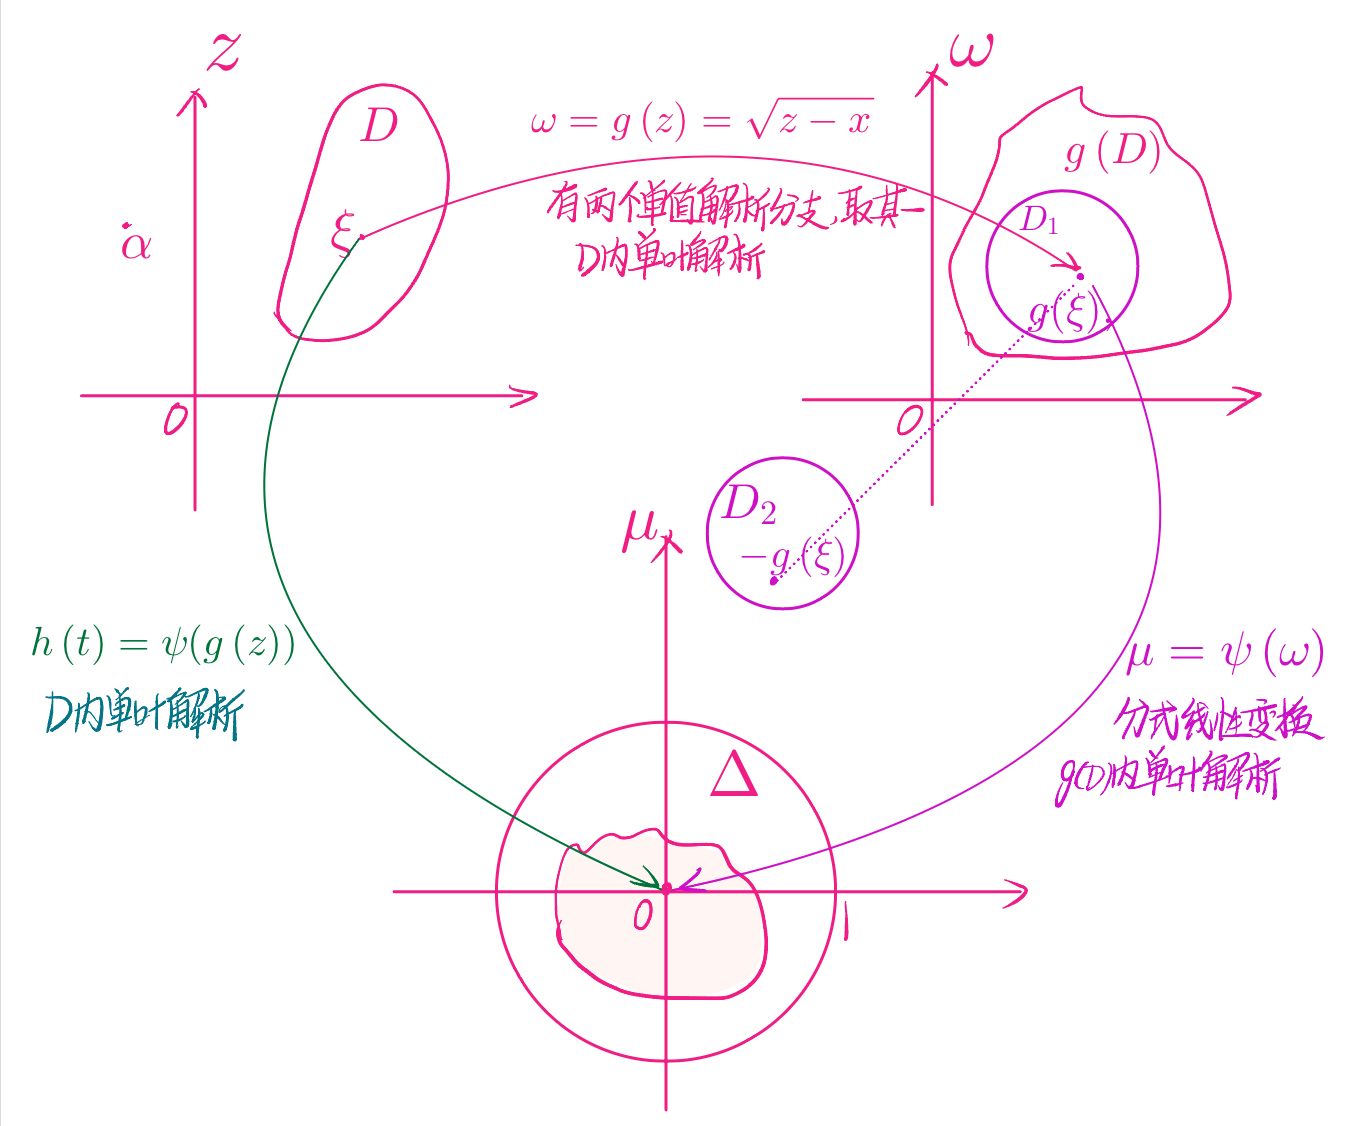
\includegraphics[width=.7\linewidth]{figures/IMG_6415.png}
    \caption{\textbf{Setp.I图示}}
    \label{fig:setpi}
\end{figure}
以 $g(\xi)$为圆心做一个包含在 $g(D)$内的圆盘 $D_1$,则 \textbf{\color{magenta!90!black}$D_1$关于原点对称的圆盘 $D_2$必然不会包含在 $g(D)$内}. 这是因为 $\forall\omega_1\in D_1,\exists z_1\in D$,使得 $g(z_1)=\omega_1$,假设 $-\omega_1\in g(D)$, 则 $\exists z_2\in D$,使得 $g(z_2)=-\omega_1$,即 $g(z_1)=-g(z_2), z_1,z_2\in D$, 与上述性质第二条矛盾. 

\textbf{\color{blue!50!black}构造 $\mu=\psi(\omega)$为分式线性变换,那么它\uwave{将 $g(\xi)$映为原点}, \uline{将 $g(D)$的内部映为单位圆盘的内}\newline\uline{部(不是整个单位圆盘)}.}
\begin{remark}
    \textbf{\color{red!50!black}$\mu$ 将圆盘 $D_2$的外部映成单位圆盘的内部}. 这总是可以做到的,\textbf{\color{red!50!black}只要保证两个圆盘的边界走向相反即可 (两个单位圆盘的边界走向一致时, $\mu$将 $\Delta$ 内部映成$\Delta$ 内部; 将$\Delta$ 外部映成$\Delta$ 外部; 两个单位圆盘的边界走向相反时, $\mu$将 $\Delta$ 外部映成$\Delta$ 内部; 将$\Delta$ 内部映成$\Delta$ 外部)}.
\end{remark}
将 $\mu=\psi(\omega)$和 $\omega=g(z)$复合后得到的函数 \uline{$h(z)=\psi(g(z))$在$D$内单叶解析},且
\[h(\xi)=\psi(g(\xi))=0.\]
但是 $h^\prime(\xi)$不一定大于零,所以不妨设 $h^\prime(\xi)=r\cdot e^{i\theta}$, 则 $e^{-i\theta}h^\prime(\xi)=r>0$.那么令 $\varphi(z)=e^{-i\theta}h(z)$,则 \uline{$\varphi^\prime(\xi)>0$},所以由上述划线部分知,$\varphi(z)$在 $D$内满足 $\mathscr{F}$的四个条件,从而 $\varphi\in\mathscr{F}$,则 $\mathscr{F}\neq \emptyset$.

由于 $g(D)$是圆盘 $D_2$外部的一部分,则由上述评注知, $g(D)$ 被 $\mu$ 映成单位圆盘内部的一部分. $\forall f\in\mathscr{F}, |f(z)|\leqslant 1$ 一致有界, 由 Montel定理知 $\mathscr{F}$是正规族.
\subsection{第二步: 证明 \texorpdfstring{$\sup_{f\in \mathscr{F}} f^\prime (\xi)$}.是有限数且它可在 \texorpdfstring{$D$}.内取到}\label{subsec:setp2}
补充结论: 上确界的一般性结论: $a=\sup S\implies \exists \{x_n\}\subset S$,使得 $\lim_{n\to\infty}x_n=a$.

设 $\sup_{f\in\mathscr{F}}f^\prime (\xi)=m\leqslant +\infty$ ($m>0$因 $f^\prime(\xi)>0$).则存在 $\{f_n\}\subset \mathscr{F}$,使得 $\lim_{n\to\infty}f^\prime_n (\xi)=m$.
因 $\mathscr{F}$是正规族,故
\begin{eq}\label{eq:1.1.1}
    \exists \{f_{n_k}\}\subset \{f_n\}\text{使得} f_{n_k}\overset{d}{\to}f\overset{(a)}{\implies} f^\prime_{n_k}\to f^\prime \overset{(b)}{\implies} \lim_{k\to\infty}f^\prime_{n_k}(\xi)=f^\prime(\xi).
\end{eq}
其中 $(a)$是因为\textbf{\color{red}原函数列内闭一致收敛那么导函数列也必内闭一致收敛 (由Cauchy积分公式证明)}; $d$表示内闭一致收敛; $(b)$为定义.
\begin{eq}
\label{eq:1.1.2}
    \text{因} \lim_{n\to\infty}f^\prime_n (\xi)=m, \text{则} \lim_{k\to\infty}f_{n_k}^\prime (\xi)=m.
\end{eq}
因此, 结合\textbf{\eqref{eq:1.1.1}}、\textbf{\eqref{eq:1.1.2}}可得 $f^\prime(\xi)=m$. 又由$\mathscr{F}$的定义知, $f^\prime(\xi)=m>0$.

因为 $f$为单叶解析函数列内闭一致收敛的极限函数,由 定理, $f$要么是单叶解析函数, 要么是常数,但由于 $f^\prime(\xi)>0$,故 $f$不能是常数,所以 $f$是单叶函数, $m=f^\prime(\xi)<+\infty$.
注意到,
\begin{eq}
    f(\xi) &=\lim_{k\to\infty}f_{n_k}(\xi)=0 ,\\ 
    |f(z)| &=\left|\lim_{k\to\infty}f_{n_k}(z)\right|\overset{(c)}{=}\lim_{k\to\infty}\left|f_{n_k}(z)\right|\overset{(d)}{\leqslant} 1.
\end{eq}
其中, $(c)$表示取模运算与极限运算次序可交换,因为取模运算是连续的; $(d)$表示极限只能保非严格不等式.下面排除 $|f(z)|=1$的情形. (反证法) 若 $|f(z)|=1$, 注意到 \textbf{模(实部)(虚部)(辐角)为常数的解析函数必为常数},则 $f$为常数,矛盾,因而 $|f(z)|<1$.
故 $f\in\mathscr{F}$,且 $f$是 $\mathscr{F}$中导数取得最大值的那一个.
\subsection{第三步: 证明上面找到的 \texorpdfstring{$f$}.就是要找的映满的共形映射,即\texorpdfstring{$f(D)=\{\omega\colon |\omega|<1\}$}.}\label{subsec:setp3}
\begin{figure}[htb]
    \centering
    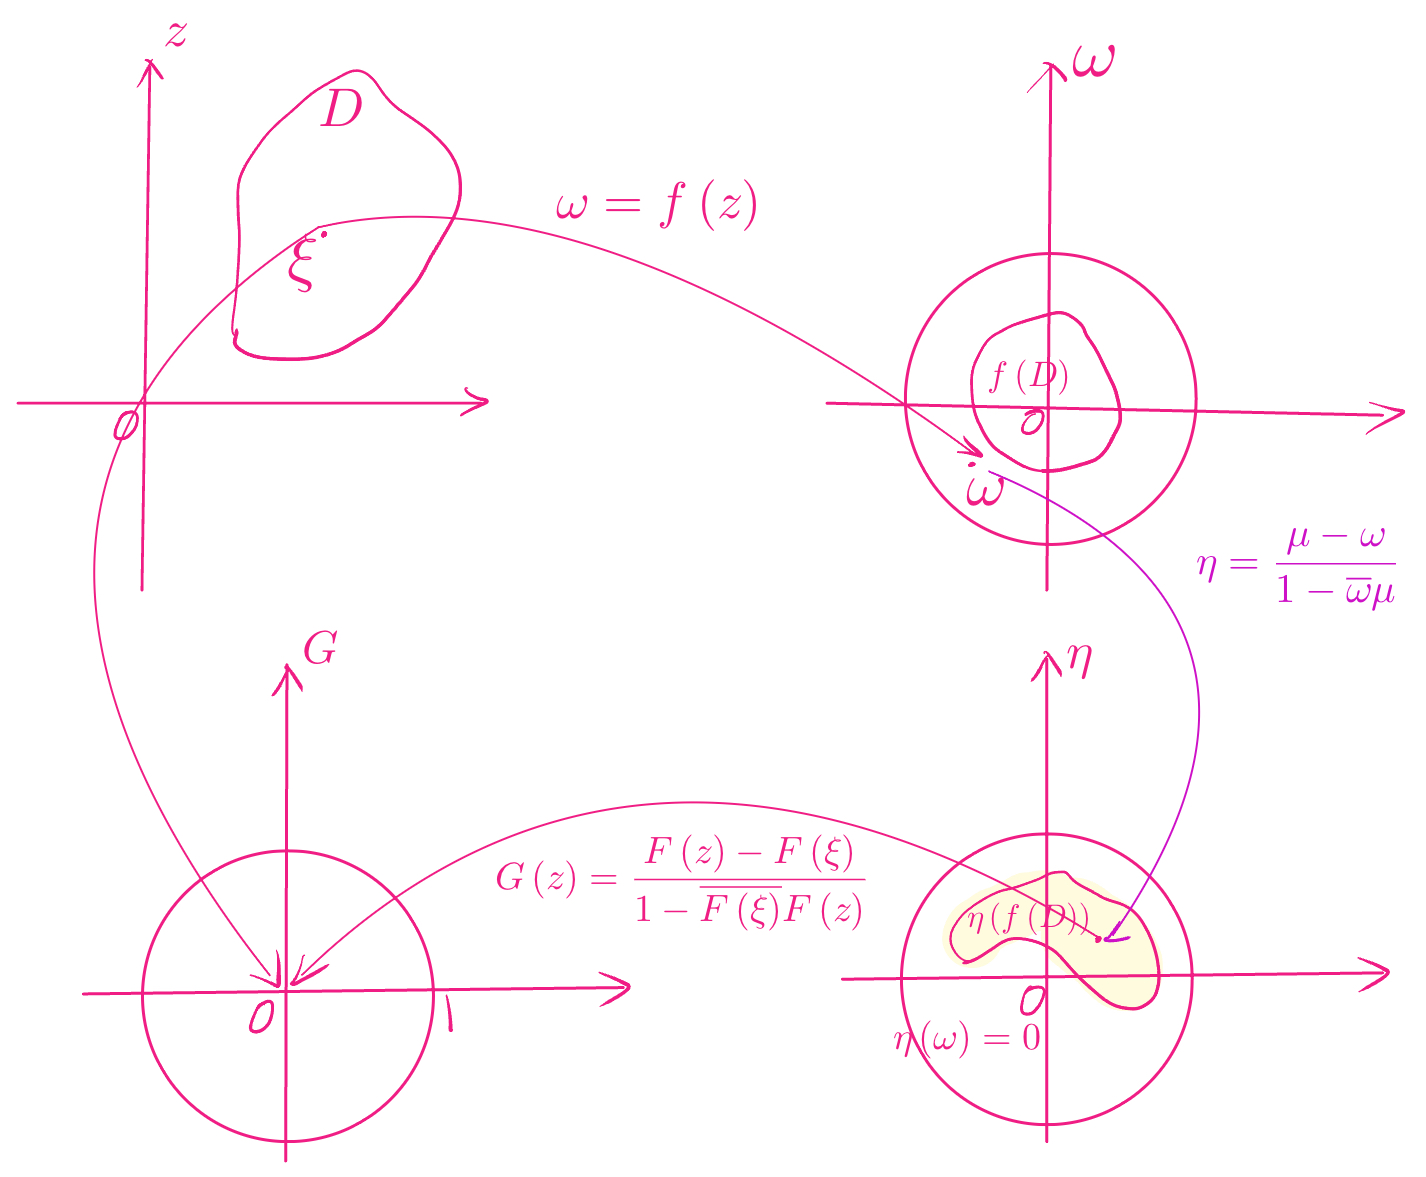
\includegraphics[width=.7\linewidth]{figures/IMG_6416.png}
    \caption{Step.III 图示}
    \label{fig:setpiii}
\end{figure}
(反证法) 设 $f(D)\neq \Delta$,即存在 $\omega\in\Delta\backslash f(D)$,取之构成分式线性变换 
\begin{eq}
    \label{eq:eta}
    \eta=\frac{f(z)-\omega}{1-\overline{\omega}f(z)}=\frac{\mu-\omega}{1-\mu\omega},
\end{eq}
则\textbf{\color{magenta}该分式线性变换将 $\omega$平面单位圆盘内的区域映成 $\eta$平面单位圆盘内的区域 (不含原点,因 $\eta(\omega)=0$, 但$\omega\not\in f(D)$)}.

设 
\begin{eq}
    \label{eq:F}
    F(z)=\sqrt{\frac{f(z)-\omega}{1-\overline{\omega}f(z)}},
\end{eq}
我们断言, $F(z)$在 $D$内单叶解析.
因 $F(z)$在 $D$内无零点,由引理可知, $F(z)$在 $D$内有单值解析分支,不妨取其一表为 $F(z)$. 若 $F(z_1)=F(z_2)$,则
\begin{eq}
    \label{eq:1.1.4}
    \frac{f(z_1)-\omega}{1-\overline{\omega}f(z_1)}=\frac{f(z_2)-\omega}{1-\overline{\omega}f(z_2)}\implies f(z_1)=f(z_2)\overset{f\text{单叶解析}}{\implies} z_1=z_2.
\end{eq}
故 \uline{$F(z)$在 $D$内是单叶解析的.}
且 \uline{\color{magenta}$|F(z)|<1$}.但这不足以使 $F(z)\in\mathscr{F}$,这是因为 $F(\xi)\not\equiv 0$.(经分式线性变换$\eta$作用后的像区域不含原点)
为此, 我们再做一次复合, 使得 
\begin{eq}
    \label{eq:G}
    G(z)=e^{-i\theta}\cdot \frac{F(z)-F(\xi)}{1-\overline{F(\xi)}F(z)},\text{其中} e^{-i\theta}=\frac{F^\prime (\xi)}{|F^\prime(\xi)|},
\end{eq}
这是因为由 \textbf{\ref{subsec:setp1}} 知 
\begin{eq*}
    e^{-i\theta}=\frac{h^\prime(\xi)}{|h^\prime(\xi)|}=\frac{F^\prime (\xi)}{|F^\prime(\xi)|}
\end{eq*}
($h$到 $F$只做了一次分式线性变换而没有旋转,因而不改变辐角).这样即可得到 $G(\xi)=0$,且 $G^\prime (\xi)>0$ ; 又$G$在 $F$基础上做旋转, 不改变模长, $|G(z)|=|F(z)|<1$ ($G$将 $F(\xi)$变为原点; ).故 $G(z)\in \mathscr{F}$.

又由于
\begin{eq}
    \label{eq:1.1.5}
    G^\prime(\xi)=\frac{|F^\prime (\xi)|}{1-|F(\xi)|^2}=\frac{1+|\omega|}{2\sqrt{\omega}}f^\prime(\xi)>f^\prime (\xi).
\end{eq}
这与\textbf{\ref{subsec:setp2}}的结论: $f^\prime(\xi)$是 $\mathscr{F}$中导数最大者矛盾,故
$G(z)$即为我们要找的映满的共形映射.

\end{proof}


















